\chapter{Results}
\label{sec:results}
The most interesting questions regarding \emph{HELM} are
\begin{itemize}
	\item How well does \emph{HELM} work compared to the iterative methods?
	\item Is \emph{HELM} able to calculate large scale power nets, for which the iterative methods do not converge?
\end{itemize}
To answer these question I have run several experiments. The ones related to the first question can be found in \secref{comparison_algorithms}. To answer the second question I added in \secref{large_scale_powernets} the results of running \emph{HELM} on the german power net in a certain configuration, for which the iterative algorithms do not converge.

\section{Comparison of the Load-flow Algorithms}
\label{sec:comparison_algorithms}

\begin{figure}
	\centering
	
\includegraphics[scale=0.7]{figures/comparison_runtime}
	\caption[Comparison, average runtime]{Average runtime of the algorithms for several power nets}
	\label{fig:comparison_runtime}
\end{figure}

\begin{figure}
	\centering
	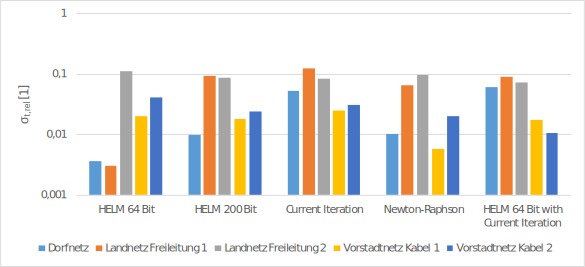
\includegraphics[scale=0.7]{figures/comparison_deviation}
	\caption[Comparison, relative standard deviation of runtime]{Relative standard deviation of the runtime of the algorithms}
	\label{fig:comparison_deviation}
\end{figure}

\begin{figure}
	\centering
	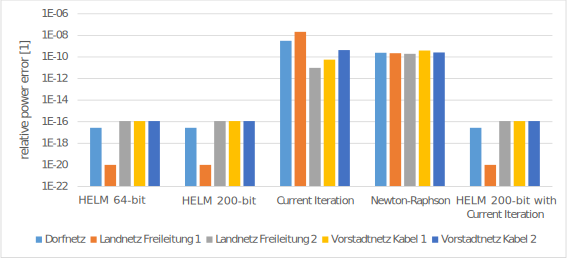
\includegraphics[scale=0.7]{figures/comparison_accuracy}
	\caption[Comparison, accuracy]{Relative power error of the algorithms}
	\label{fig:comparison_accuracy}
\end{figure}

\begin{table}
	\small
	\begin{tabularx}{\textwidth}{|X|p{1.5cm}|p{1.6cm}|p{1.5cm}|p{1.9cm}|}
		\hline
		method & target precision & maximum iterations & datatype size & maximum coefficients \\ \hline
		Current Iteration & 1e-5 & 100 & & \\ \hline
		Newton-Raphson & 1e-5 & 100 & & \\ \hline
		HELM 64 Bit & 1e-5 & & 64 & 50 \\ \hline
		HELM 200 Bit & 1e-5 & & 200 & 100 \\ \hline
		HELM 64 Bit with Current Iteration & 1e-5 & 100 & 64 & 50 \\ \hline
	\end{tabularx}
	\caption{Algorithm parameter for the comparison}
	\label{tab:comparison_parameter}
\end{table}

\section{Calculation of Large-Scale Powernets}
\label{sec:large_scale_powernets}

\section{Conclusion}